\section{Análisis multifractal}

\subsection{Relación entre multifractalidad y robustez}

El análisis multifractal provee una herramienta para examinar la estructura de una red. Ahora, se va hacer una relación entre esa medida y algunas redes. Las estrategias de ataque fueron definidas en el capitulo \ref{cap5}.

Las redes de estudio son:

\begin{enumerate}
    \item Red A: Red libre de escala 8000 nodos
    \item Red B: Red de mundo pequeño 5000 nodos, probabilidad de reconexión 10\%
    \item Red C: Red aleatoria 1991 nodos
    \item Red D: Red real bacteria C.elegans
    \item Red E: Red fractal (1,3)-flower
\end{enumerate}

Debido a que se debe ejecutar el análisis de multifractalidad a medida que se pierde un porcentaje de nodos, se utiliza el algoritmo SandBox.

\subsubsection{Red libre de escala}

\begin{figure}[H]
    \centering
    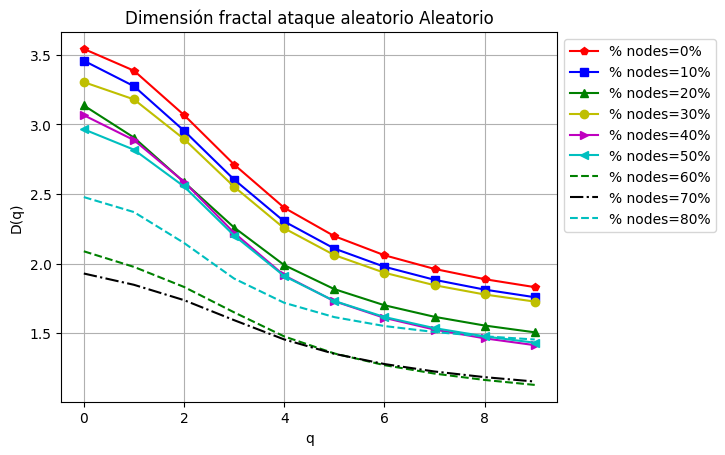
\includegraphics[scale=0.7]{Capitulo6MultifractalidadYRobustez/imagenes/grafica_DqRandom20180512_143117ScaleFree8000Nodes.png}
    \caption{Análisis de multifractalidad de red libre de escala a ataque aleatorio }
\end{figure}

\begin{figure}[H]
    \centering
    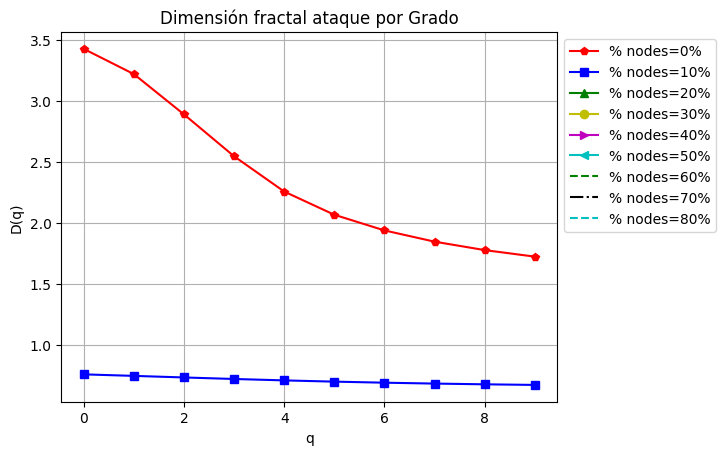
\includegraphics[scale=0.7]{Capitulo6MultifractalidadYRobustez/imagenes/grafica_DqDegree20180512_143117ScaleFree8000Nodes.png}
    \caption{Análisis de multifractalidad de red libre de escala a ataque por grado }
\end{figure}

\begin{figure}[H]
    \centering
    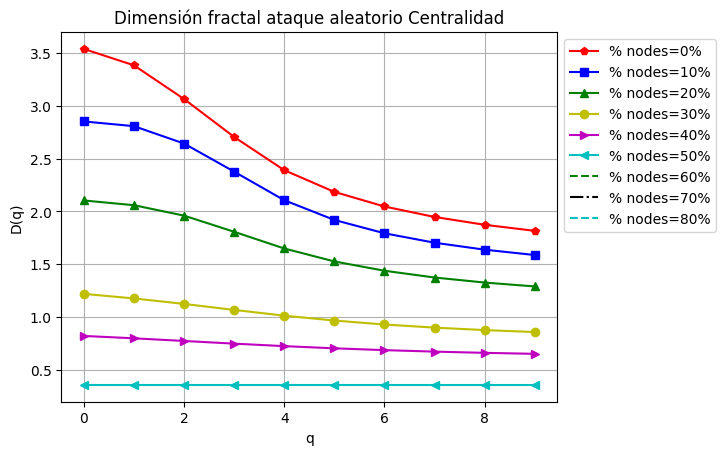
\includegraphics[scale=0.7]{Capitulo6MultifractalidadYRobustez/imagenes/grafica_DqCentrality20180512_143117ScaleFree8000Nodes.png}
    \caption{Análisis de multifractalidad de red libre de escala a ataque por centralidad }
\end{figure}


\begin{figure}[H]
    \centering
    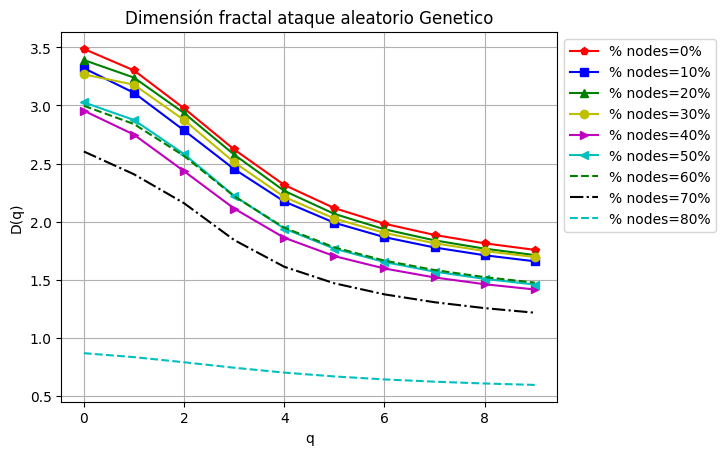
\includegraphics[scale=0.7]{Capitulo6MultifractalidadYRobustez/imagenes/grafica_DqGenetic20180512_143117ScaleFree8000Nodes.png}
    \caption{Análisis de multifractalidad de red libre de escala a ataque por estrategia evolutiva }
\end{figure}

\begin{figure}[H]
    \centering
    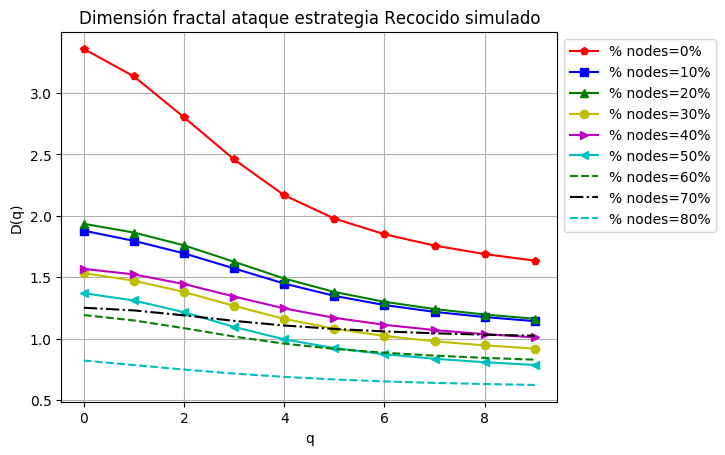
\includegraphics[scale=0.7]{Capitulo6MultifractalidadYRobustez/imagenes/grafica_DqSimulated20180512_143117ScaleFree8000Nodes.png}
    \caption{Análisis de multifractalidad de red libre de escala a ataque por estrategia recocida simulada }
\end{figure}


\subsubsection{Red de mundo pequeño}
\begin{figure}[H]
    \centering
    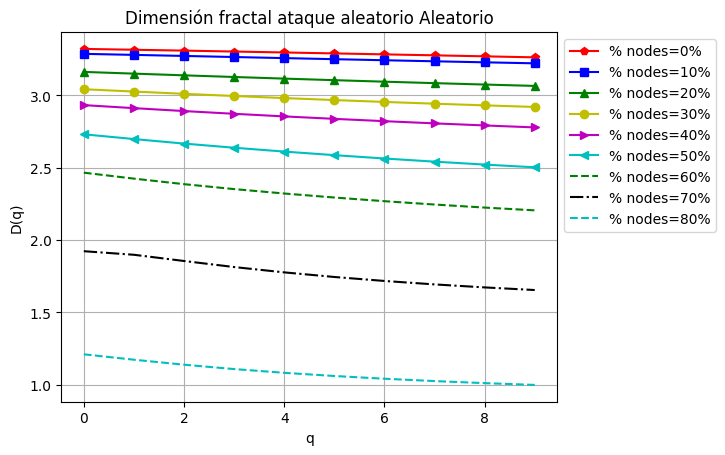
\includegraphics[scale=0.7]{Capitulo6MultifractalidadYRobustez/imagenes/grafica_DqRandom20180510_143549SmallWorld5000NodesRewire01.png}
    \caption{Análisis de multifractalidad de red de mundo pequeño ataque aleatorio }
\end{figure}

\begin{figure}[H]
    \centering
    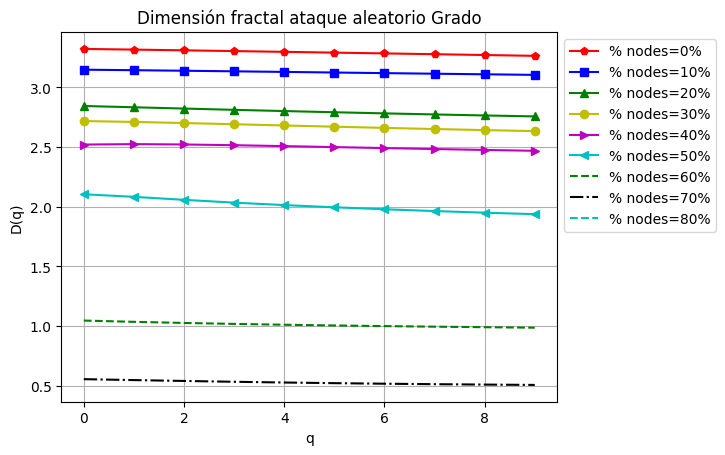
\includegraphics[scale=0.7]{Capitulo6MultifractalidadYRobustez/imagenes/grafica_DqDegree20180510_143549SmallWorld5000NodesRewire01.png}
    \caption{Análisis de multifractalidad de rred de mundo pequeño a ataque por grado }
\end{figure}

\begin{figure}[H]
    \centering
    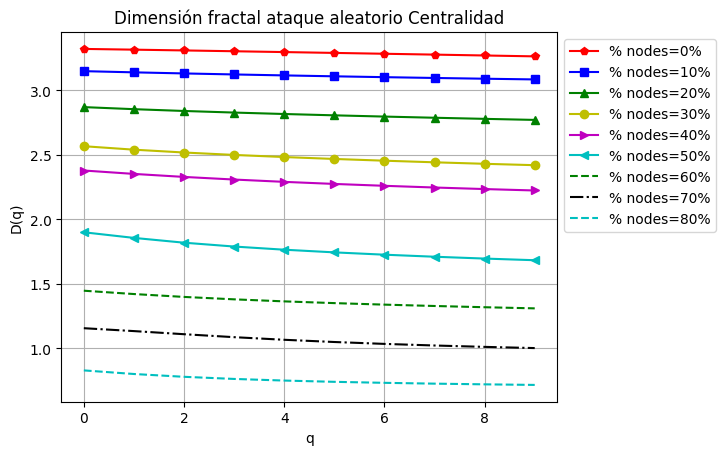
\includegraphics[scale=0.7]{Capitulo6MultifractalidadYRobustez/imagenes/grafica_DqCentrality20180510_143549SmallWorld5000NodesRewire01.png}
    \caption{Análisis de multifractalidad de red de mundo pequeño a ataque por centralidad }
\end{figure}


\begin{figure}[H]
    \centering
    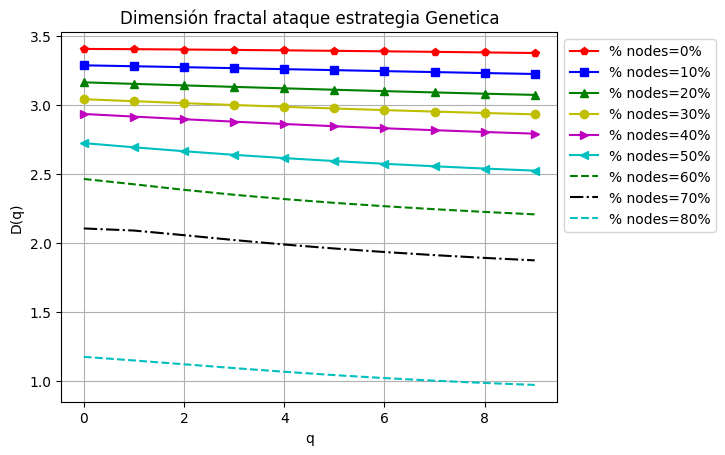
\includegraphics[scale=0.7]{Capitulo6MultifractalidadYRobustez/imagenes/grafica_DqGenetic20180510_143549SmallWorld5000NodesRewire01.png}
    \caption{Análisis de multifractalidad de red red de mundo pequeño a ataque por estrategia evolutiva }
\end{figure}

\begin{figure}[H]
    \centering
    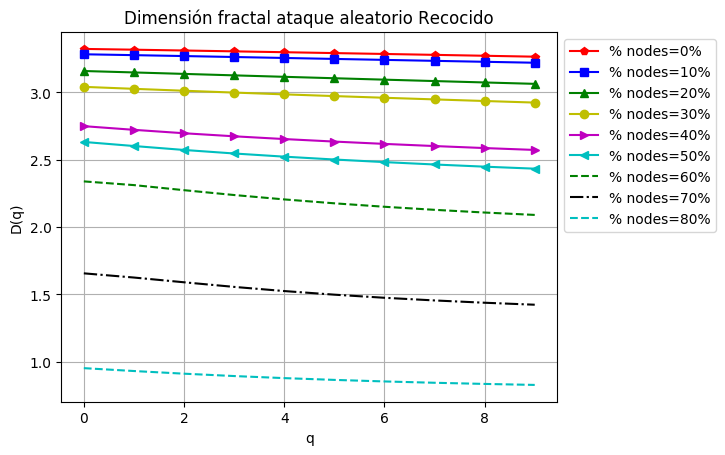
\includegraphics[scale=0.7]{Capitulo6MultifractalidadYRobustez/imagenes/grafica_DqSimulated20180510_143549SmallWorld5000NodesRewire01.png}
    \caption{Análisis de multifractalidad de red de mundo pequeño a ataque por estrategia recocida simulada }
\end{figure}

\subsubsection{Red aleatoria}
\begin{figure}[H]
    \centering
    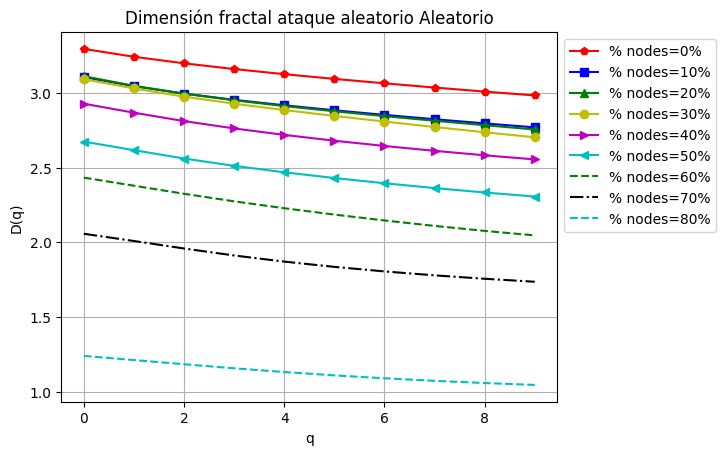
\includegraphics[scale=0.7]{Capitulo6MultifractalidadYRobustez/imagenes/grafica_DqRandom20180501_072543Random1991Nodes5939.png}
    \caption{Análisis de multifractalidad de red aleatoria a ataque aleatorio }
\end{figure}

\begin{figure}[H]
    \centering
    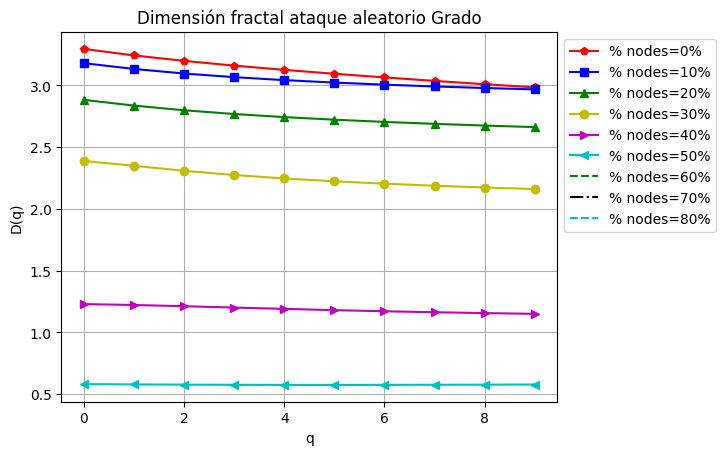
\includegraphics[scale=0.7]{Capitulo6MultifractalidadYRobustez/imagenes/grafica_DqDegree20180501_072543Random1991Nodes5939.png}
    \caption{Análisis de multifractalidad de red aleatoria a ataque por grado }
\end{figure}

\begin{figure}[H]
    \centering
    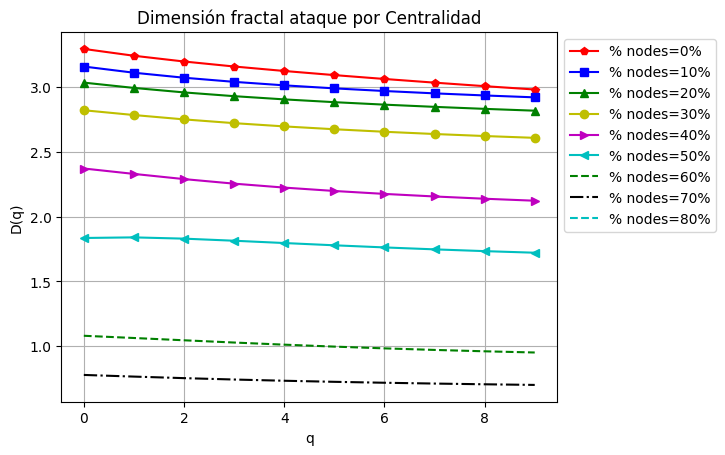
\includegraphics[scale=0.7]{Capitulo6MultifractalidadYRobustez/imagenes/grafica_DqCentrality20180501_072543Random1991Nodes5939.png}
    \caption{Análisis de multifractalidad de red aleatoria a ataque por centralidad }
\end{figure}


\begin{figure}[H]
    \centering
    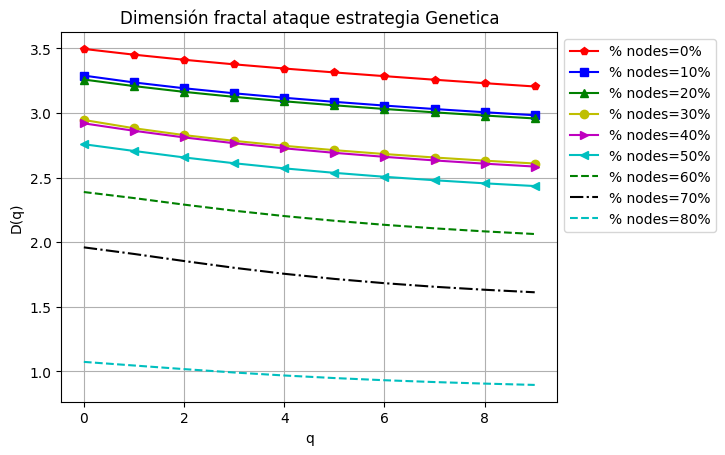
\includegraphics[scale=0.7]{Capitulo6MultifractalidadYRobustez/imagenes/grafica_DqGenetic20180501_072543Random1991Nodes5939.png}
    \caption{Análisis de multifractalidad de red red aleatoria a ataque por estrategia evolutiva }
\end{figure}

\begin{figure}[H]
    \centering
    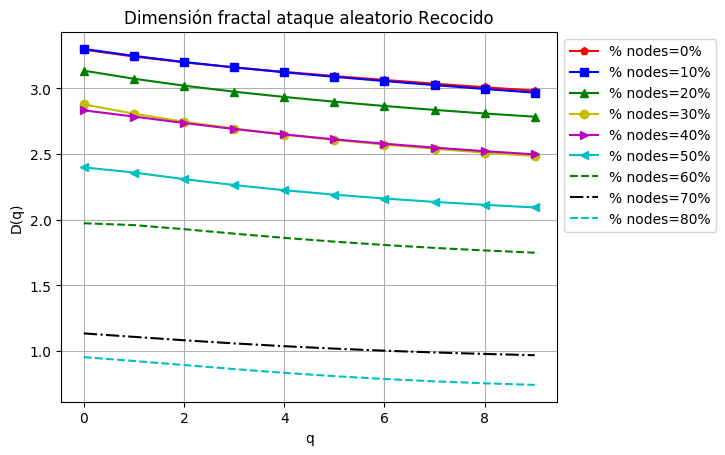
\includegraphics[scale=0.7]{Capitulo6MultifractalidadYRobustez/imagenes/grafica_DqSimulated20180501_072543Random1991Nodes5939.png}
    \caption{Análisis de multifractalidad de red red aleatoria a ataque por estrategia recocida simulada }
\end{figure}

\subsubsection{Red real}

\begin{figure}[H]
    \centering
    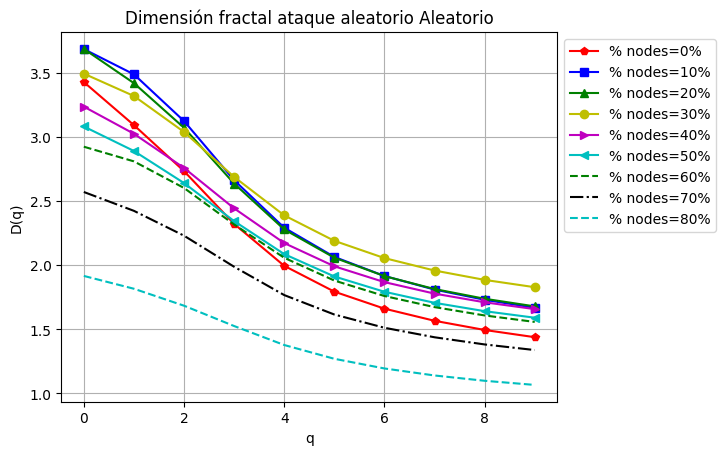
\includegraphics[scale=0.7]{Capitulo6MultifractalidadYRobustez/imagenes/grafica_DqRandom20180508_020345Celengs.png}
    \caption{Análisis de multifractalidad de red real Celegens a ataque aleatorio}
\end{figure}

\begin{figure}[H]
    \centering
    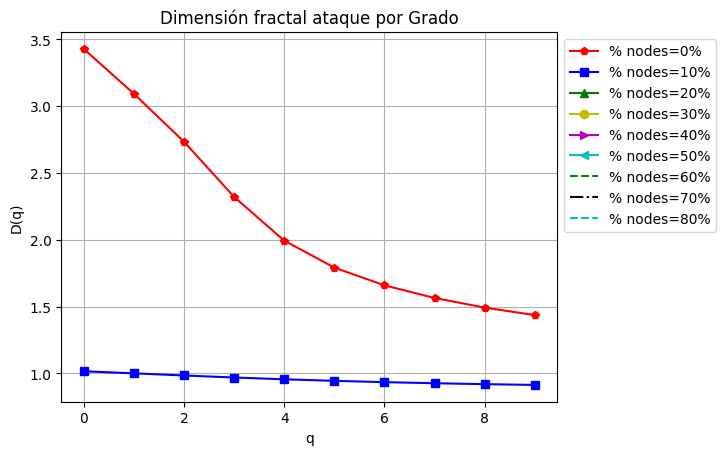
\includegraphics[scale=0.7]{Capitulo6MultifractalidadYRobustez/imagenes/grafica_DqDegree20180508_020345Celengs.png}
    \caption{Análisis de multifractalidad de red real Celegens a ataque por grado}
\end{figure}

\begin{figure}[H]
    \centering
    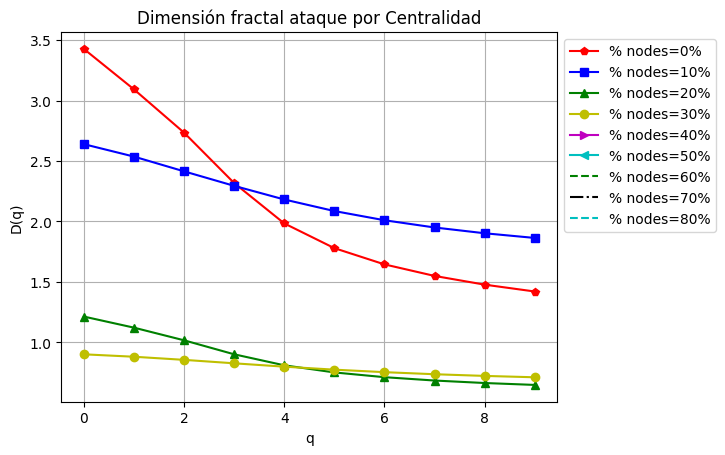
\includegraphics[scale=0.7]{Capitulo6MultifractalidadYRobustez/imagenes/grafica_DqCentrality20180508_020345Celengs.png}
    \caption{Análisis de multifractalidad de red real Celegens a ataque por centralidad}
\end{figure}


\begin{figure}[H]
    \centering
    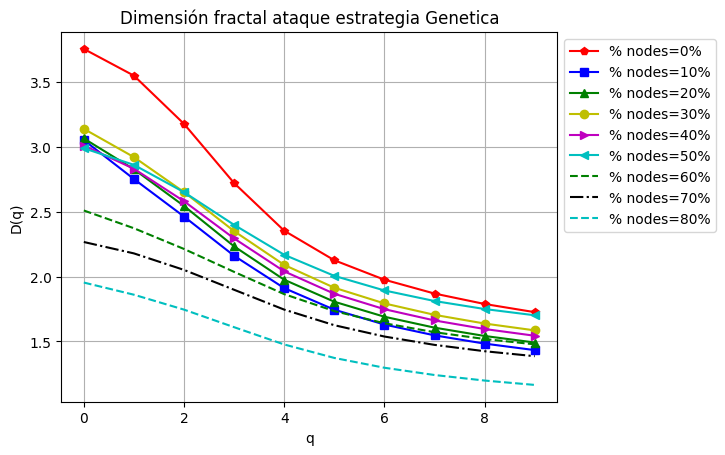
\includegraphics[scale=0.7]{Capitulo6MultifractalidadYRobustez/imagenes/grafica_DqGenetic20180508_020345Celengs.png}
    \caption{Análisis de multifractalidad de red real Celegens a ataque por estrategia evolutiva}
\end{figure}

\begin{figure}[H]
    \centering
    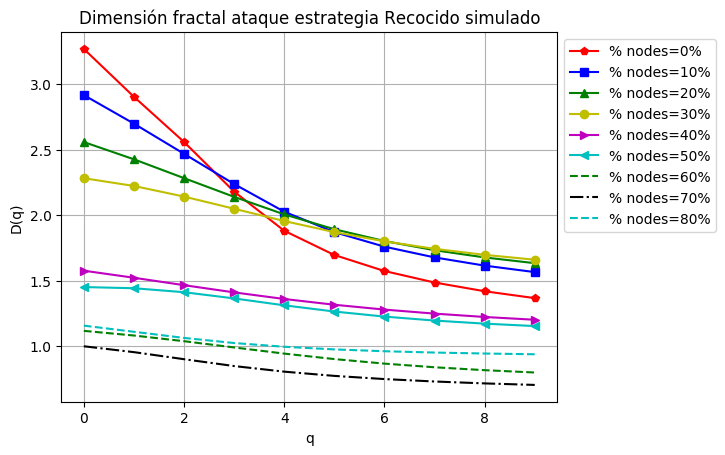
\includegraphics[scale=0.7]{Capitulo6MultifractalidadYRobustez/imagenes/grafica_DqSimulated20180508_020345Celengs.png}
    \caption{Análisis de multifractalidad de red real Celegens a ataque por estrategia recocida simulada }
\end{figure}

\subsubsection{Red fractal}
\begin{figure}[H]
    \centering
    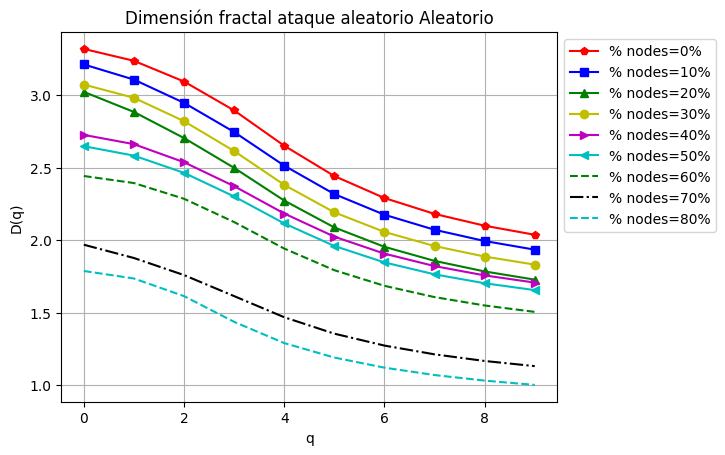
\includegraphics[scale=0.7]{Capitulo6MultifractalidadYRobustez/imagenes/grafica_DqRandom20180501_151350floweru1v3.png}
    \caption{Análisis de multifractalidad de red libre de escala a ataque aleatorio }
\end{figure}

\begin{figure}[H]
    \centering
    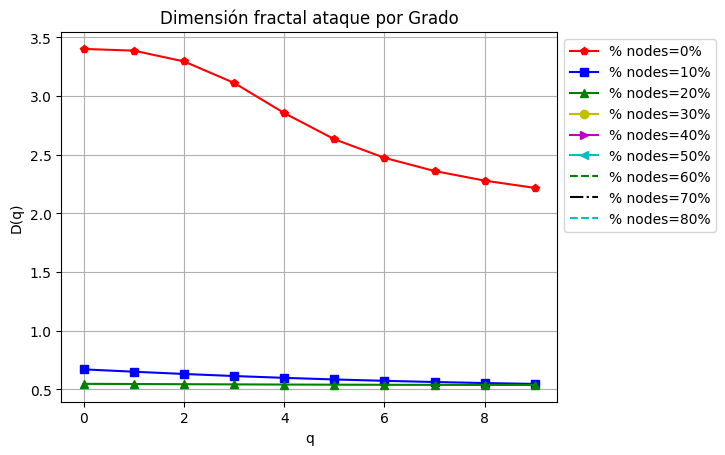
\includegraphics[scale=0.7]{Capitulo6MultifractalidadYRobustez/imagenes/grafica_DqDegree20180501_151350floweru1v3.png}
    \caption{Análisis de multifractalidad de red (1,3)-flower a ataque por grado }
\end{figure}

\begin{figure}[H]
    \centering
    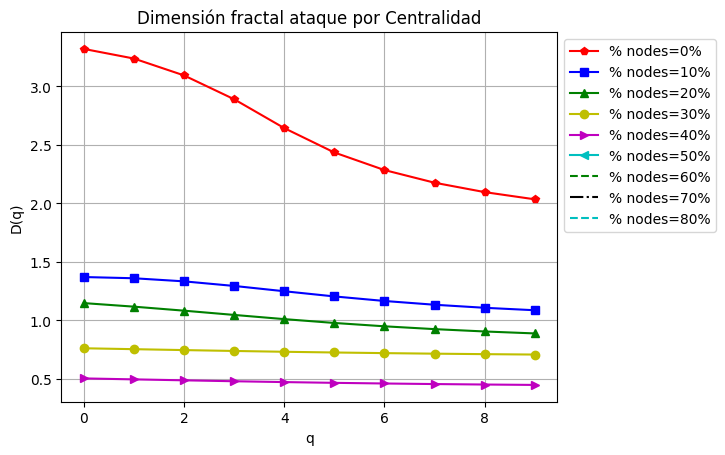
\includegraphics[scale=0.7]{Capitulo6MultifractalidadYRobustez/imagenes/grafica_DqCentrality20180501_151350floweru1v3.png}
    \caption{Análisis de multifractalidad de red (1,3)-flower a ataque por centralidad }
\end{figure}


\begin{figure}[H]
    \centering
    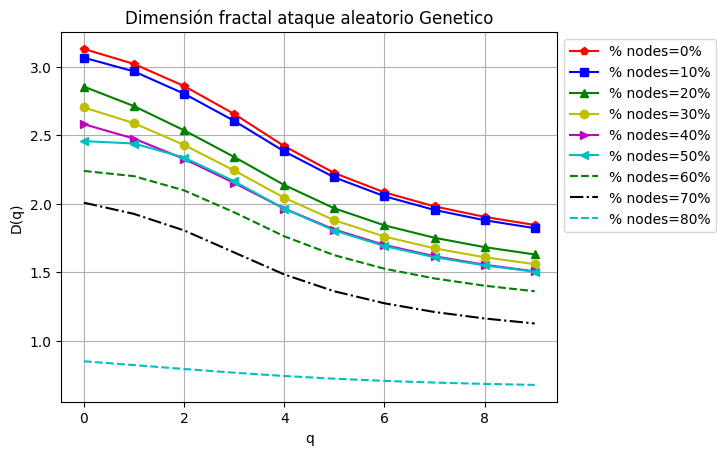
\includegraphics[scale=0.7]{Capitulo6MultifractalidadYRobustez/imagenes/grafica_DqGenetic20180501_151350floweru1v3.png}
    \caption{Análisis de multifractalidad de red (1,3)-flower a ataque por estrategia evolutiva }
\end{figure}

\begin{figure}[H]
    \centering
    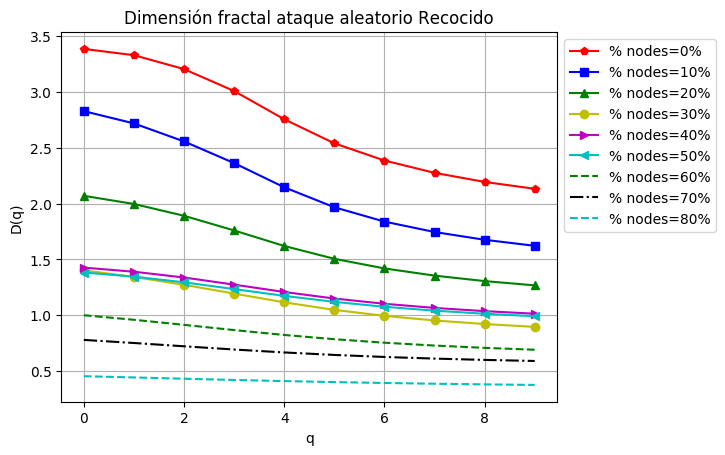
\includegraphics[scale=0.7]{Capitulo6MultifractalidadYRobustez/imagenes/grafica_DqSimulated20180501_151350floweru1v3.png}
    \caption{Análisis de multifractalidad de red (1,3)-flowera ataque por estrategia recocida simulada }
\end{figure}

\subsection{Discusión de resultados}

La relación entre multifractalidad y robustez está dada en como se comporta la dimensión fractal de la red a medida que pierde nodos.

La estrategia que más efectos produce son las estrategias de ataque por grado y por centralidad, ya que estas tienden a desintegrar la red. El efecto es tan fuerte, que eliminados un 20\% a 30\% de los nodos, no es posible aplicar los algoritmos de análisis multifractal.

Las estrategias de ataque por algoritmos de Inteligencia Artificial, no tienen un efecto tan evidente como lo tienen la centralidad o el grado. Sin embargo, muestran mayor efecto en la redes que las estrategia aleatoria.

Con respecto a las redes de mundo pequeño, se observa que estas conservan su estructura a medida que pierde nodos, lo que muestra que su estructura interna permanece intacta ante diferentes estrategias de ataque.

Para las redes aleatorias, libres de escala, reales y fractales, se encuentra que pierden su estructura a medida que pierden nodos, pasando de ser objetos multifractales a monofractales. Esto se debe a que estas presentan en mayor o menor medida hubs, los cuales estructuralmente son los centros de estructuras internas, que a medida que se pierden la red se va tornando más uniforme.

En todos los casos, la dimensión fractal tiende hacia 1 a medida que la red pierde nodos. Una dimensión fractal 1, indica que la red pasa de ser un conjunto n-dimensional a uno unidimensional.